\documentclass[10pt,a4paper]{article}
\usepackage[margin=1.8cm,top=1.5cm,bottom=1.6cm]{geometry}
\usepackage[T1]{fontenc}
\usepackage[utf8]{inputenc}
\usepackage{lmodern}
\usepackage{microtype}
\usepackage{booktabs}
\usepackage{caption}
\usepackage{subcaption}
\usepackage{tikz}
\usepackage[hidelinks]{hyperref}

\definecolor{weekday}{HTML}{2A78D6}
\definecolor{weekend}{HTML}{EB6834}
\definecolor{grid}{HTML}{E1E0D9}
\captionsetup{font=small,labelfont=bf,skip=3pt}
\setlength{\parskip}{3pt}
\setlength{\parindent}{0pt}
\pagestyle{empty}

\title{\vspace{-0.8cm}\textbf{Stockholm Public Transport Delay Analytics Using Apache Spark}}
\author{Group 67: Hieu Vu, Rong Jin, Serban}
\date{\vspace{-0.9cm}}

\begin{document}
\maketitle
\thispagestyle{empty}

\section*{1\quad Goal and dataset}
We analyse one month of real-time data from Stockholm's public transport (SL) to answer four questions:
which lines have the highest average delays, which stations are most often delayed, during which hours
delays are worst, and how weekdays and weekends differ.

The data comes from Trafiklab's \textbf{KoDa} archive of SL's open feeds
(\href{https://www.trafiklab.se/api/trafiklab-apis/koda/}{\texttt{trafiklab.se/api/trafiklab-apis/koda}}, free API key; too large to include, but
\texttt{scripts/download\_koda.py} downloads it). We use two parts:
\textbf{GTFS-RT TripUpdates}, a snapshot of every running trip's arrival times and delays taken about
every 14 seconds (around 6,000 files and 4.5\,GB unpacked per day), and the \textbf{static GTFS}
timetable valid on each day, which turns trip and stop ids into line numbers, station names, coordinates
and scheduled times. We downloaded 7--8 and 12--27 September 2026. Days with both parts give
\textbf{16 service days} (12 weekdays, 4 weekend days): \textbf{9.5 million vehicle stops} on 481,507
trips, 578 lines and 5,891 stations.

\section*{2\quad Methodology}
\textbf{Storage and tools.} A single-node HDFS (Hadoop 3.4.3) holds all data as Parquet, partitioned by
day (and by hour for the raw delays); processing is PySpark~4; the dashboard is Plotly Dash.

\textbf{Ingestion} (\texttt{hdfs-ingression.py}). Timetable tables are converted from CSV to Parquet,
one copy per day. The trip update snapshots are parsed from protobuf; since each snapshot repeats every
trip with a revised estimate, only the newest row per trip, service day and stop is kept within each hour
(about 96$\times$ fewer rows, with no information lost). A \texttt{-{}-day-by-day} mode unpacks, ingests
and deletes one date at a time, so the 85\,GB month fits on a laptop.

\textbf{Preprocessing} (Spark, \texttt{spark-preprocessing.py}). (1)~A window keeps the newest row
per (trip, stop, service day) across all hour folders, as one stop appears in several hours while its
trip runs; the service day is part of the key because SL reuses trip ids. (2)~Stops whose time was still
in the future when last seen never happened (e.g.\ cancelled) and are dropped. (3)~The delay is the
departure delay at a trip's first stop (vehicles arrive early and wait) and the arrival delay elsewhere;
missing values and delays outside $-15$\,min to $+2$\,h are removed. (4)~Each stop is joined with the
\emph{same day's} timetable (trips, routes, stops, stop\_times) and platforms are mapped to their parent
station. (5)~We add the scheduled Stockholm hour, weekday/weekend, transport mode and a \emph{late} flag
($\geq$3 minutes). 15.3\,M hourly rows become 10.1\,M distinct stops and 9.5\,M joined stop events; the
rows lost in the join belong almost entirely to days whose timetable was not downloaded.

\textbf{Analytics} (Spark, \texttt{spark-analytics.py}). For lines, stations, hours, day types, transport
modes and one-minute delay bins we compute the number of stops, mean, exact median and 90th percentile
delay, and the share of late stops. Lines are grouped by \texttt{route\_id} and stations by
\texttt{station\_id}, not by name (line ``14'' is both a metro and a ferry; ``Slussen'' is five
stations). Only lines with $\geq$100 and stations with $\geq$50 stops per day are ranked. Results are
written to HDFS and exported as CSV for the dashboard (\texttt{dashboard.py}).

\textbf{Verification.} Both Spark stages were reimplemented independently in pandas and compared value by
value (all rows and columns identical), and sampled stops were traced back to the raw protobuf files.
This caught real bugs, e.g.\ a station split in two after its coordinates moved between timetables.

\section*{3\quad Results}
On average a stop is \textbf{92\,s late} (median 60\,s) and \textbf{20.3\% of stops are 3+ minutes late};
a quarter of stops are early and 1.5\% are 10+ minutes late.

\begin{figure}[h]
\centering
\begin{subfigure}[t]{0.49\linewidth}
\centering
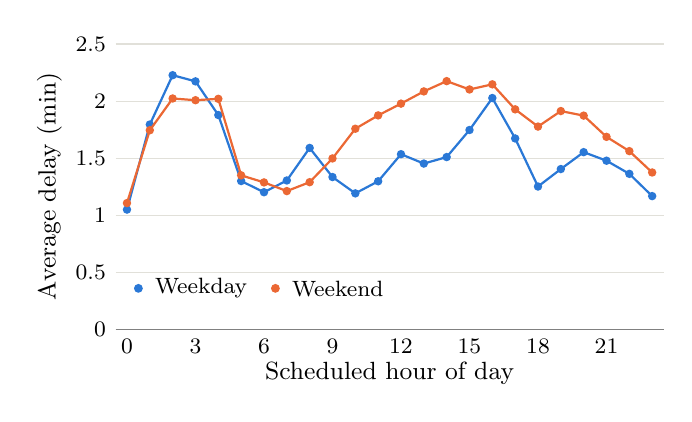
\begin{tikzpicture}[x=0.29cm, y=1.45cm, font=\footnotesize]
\foreach \v in {0,0.5,...,2.5} {\draw[grid] (-0.5,\v) -- (23.5,\v); \node[left] at (-0.5,\v) {\v};}
\foreach \h in {0,3,...,21} {\node[below] at (\h,0) {\h};}
\draw[gray] (-0.5,0) -- (23.5,0);
\draw[weekday, thick] plot[mark=*, mark size=1.1pt] coordinates {(0,1.050) (1,1.795) (2,2.227) (3,2.173) (4,1.878) (5,1.300) (6,1.202) (7,1.305) (8,1.590) (9,1.335) (10,1.192) (11,1.298) (12,1.535) (13,1.453) (14,1.510) (15,1.747) (16,2.027) (17,1.673) (18,1.252) (19,1.405) (20,1.553) (21,1.478) (22,1.363) (23,1.168)};
\draw[weekend, thick] plot[mark=*, mark size=1.1pt] coordinates {(0,1.107) (1,1.745) (2,2.023) (3,2.008) (4,2.020) (5,1.350) (6,1.288) (7,1.212) (8,1.290) (9,1.498) (10,1.758) (11,1.875) (12,1.978) (13,2.085) (14,2.175) (15,2.102) (16,2.147) (17,1.928) (18,1.777) (19,1.913) (20,1.873) (21,1.687) (22,1.562) (23,1.375)};
\node[below] at (11.5,-0.2) {\small Scheduled hour of day};
\node[rotate=90] at (-3.4,1.25) {\small Average delay (min)};
\fill[weekday] (0.5,0.36) circle (1.6pt); \node[right] at (0.8,0.36) {Weekday};
\fill[weekend] (6.5,0.36) circle (1.6pt); \node[right] at (6.8,0.36) {Weekend};
\end{tikzpicture}
\caption{Average delay by hour, all modes.}
\label{fig:hourly}
\end{subfigure}\hfill
\begin{subfigure}[t]{0.49\linewidth}
\centering
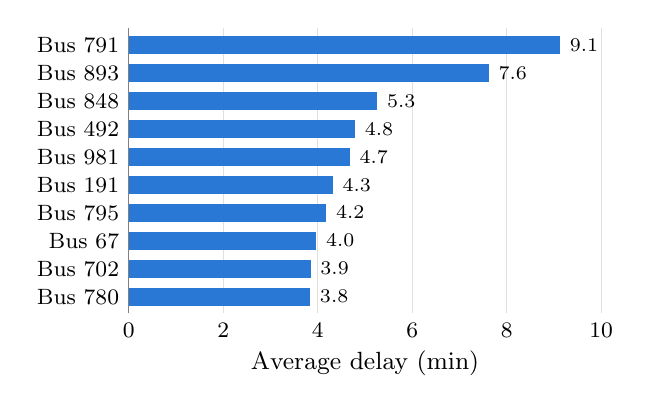
\begin{tikzpicture}[x=0.6cm, y=0.355cm, font=\footnotesize]
\foreach \m in {0,2,...,10} {\draw[grid] (\m,-0.6) -- (\m,9.6); \node[below] at (\m,-0.6) {\m};}
\fill[weekday] (0,8.68) rectangle (9.13,9.32); \node[left] at (0,9) {Bus 791}; \node[right, font=\scriptsize] at (9.13,9) {9.1};
\fill[weekday] (0,7.68) rectangle (7.62,8.32); \node[left] at (0,8) {Bus 893}; \node[right, font=\scriptsize] at (7.62,8) {7.6};
\fill[weekday] (0,6.68) rectangle (5.26,7.32); \node[left] at (0,7) {Bus 848}; \node[right, font=\scriptsize] at (5.26,7) {5.3};
\fill[weekday] (0,5.68) rectangle (4.79,6.32); \node[left] at (0,6) {Bus 492}; \node[right, font=\scriptsize] at (4.79,6) {4.8};
\fill[weekday] (0,4.68) rectangle (4.68,5.32); \node[left] at (0,5) {Bus 981}; \node[right, font=\scriptsize] at (4.68,5) {4.7};
\fill[weekday] (0,3.68) rectangle (4.32,4.32); \node[left] at (0,4) {Bus 191}; \node[right, font=\scriptsize] at (4.32,4) {4.3};
\fill[weekday] (0,2.68) rectangle (4.18,3.32); \node[left] at (0,3) {Bus 795}; \node[right, font=\scriptsize] at (4.18,3) {4.2};
\fill[weekday] (0,1.68) rectangle (3.97,2.32); \node[left] at (0,2) {Bus 67}; \node[right, font=\scriptsize] at (3.97,2) {4.0};
\fill[weekday] (0,0.6799999999999999) rectangle (3.85,1.32); \node[left] at (0,1) {Bus 702}; \node[right, font=\scriptsize] at (3.85,1) {3.9};
\fill[weekday] (0,-0.32) rectangle (3.84,0.32); \node[left] at (0,0) {Bus 780}; \node[right, font=\scriptsize] at (3.84,0) {3.8};
\draw[gray] (0,-0.6) -- (0,9.6);
\node[below] at (5,-1.6) {\small Average delay (min)};
\end{tikzpicture}
\caption{The ten lines with the highest average delay.}
\label{fig:lines}
\end{subfigure}
\caption{Delays by hour and by line, 16 service days in September 2026.}
\vspace{-6pt}
\end{figure}

\textbf{Lines (Fig.~\ref{fig:lines}).} The ten most delayed lines are all buses: bus 791 averages
9.1\,min late and is late at 85\% of its stops, followed by buses 893 (7.6\,min) and 848 (5.3\,min).
Rail is far more punctual: no metro, commuter train or tram line averages more than about a minute late,
against a median of 88\,s across bus lines.

\textbf{Stations.} The stations most often 3+ minutes late are bus stops in two corridors: around
Tungelsta (Tungelsta skola 76.5\%, Mulstavägen 66.8\%), served by buses 835, 848 and 893, and in
Östermalm on bus 67 (Skeppargatan, Runebergsplan, Historiska museet, Strandvägen, all around 60--62\%).
Delays accumulate along a trip, so a station's punctuality mostly reflects the lines through it. The
busiest stations by vehicle stops are bus terminals (Londonviadukten 2,299 stops/day, Henriksdal 2,199)
and T-Centralen (1,868, all seven metro lines); being busy does not imply being late (Henriksdal 35\%
late, T-Centralen 2\%).

\textbf{Hours (Fig.~\ref{fig:hourly}).} On weekdays delays build through the day and peak in the afternoon
rush at 16:00 (2.0\,min, 27.6\% late), with a smaller morning peak at 08:00; 06:00 and 10:00 are the most
punctual daytime hours. The high values between 01:00 and 04:00 come from only 2.8\% of all stops.

\textbf{Weekday vs weekend.} Weekends are worse overall (108\,s vs 89\,s average; 23.2\% vs 19.7\% late),
but only because of buses, which make up 87\% of stops: every other mode is \emph{more} punctual at the
weekend (Table~\ref{tab:days}). The weekend gap is largest between 10:00 and 14:00, and the two Saturdays
were the worst days of the month.

\begin{table}[h]
\centering\small
\caption{Average delay and share of late stops by transport mode.}
\label{tab:days}
\begin{tabular}{@{}lrrrr@{}}
\toprule
 & \multicolumn{2}{c}{Average delay} & \multicolumn{2}{c}{Late ($\geq$3\,min)}\\
\cmidrule(lr){2-3}\cmidrule(l){4-5}
Mode & Weekday & Weekend & Weekday & Weekend \\
\midrule
Bus   & 98\,s & 124\,s & 21.8\% & 26.8\% \\
Ferry & 106\,s & 86\,s & 24.0\% & 20.3\% \\
Tram  & 29\,s & 24\,s & 3.3\% & 3.0\% \\
Train & 26\,s & $-5$\,s & 8.5\% & 3.5\% \\
Metro & 13\,s & 3\,s & 2.5\% & 0.9\% \\
\midrule
All   & 89\,s & 108\,s & 19.7\% & 23.2\% \\
\bottomrule
\end{tabular}
\vspace{-4pt}
\end{table}

\textbf{Limitations.} Sixteen September days (two weekends, no holidays); every vehicle stop counts the
same regardless of passengers; cancelled trips have no actual time and are not counted as delays; and the
pipeline runs on a single machine, although it is written for a cluster.

\section*{4\quad Running the code}
Requirements: Python~3.10+, Java~17 and Hadoop~3.4 (single-node HDFS; setup steps in
\texttt{README.md}). Put a KoDa API key in \texttt{.env} as \texttt{KODA\_KEY} (see \texttt{.env.example}).
\begin{verbatim}
python -m venv .venv && source .venv/bin/activate
pip install -r requirements.txt
hdfs --daemon start namenode && hdfs --daemon start datanode
python scripts/download_koda.py --start 2026-09-07 --end 2026-09-27  # to data/raw
python scripts/hdfs-ingression.py --day-by-day   # Parquet into HDFS /sl
python scripts/spark-preprocessing.py            # /sl/stop_events
python scripts/spark-analytics.py                # /sl/analytics, data/analytics
python scripts/dashboard.py                      # http://127.0.0.1:8050
\end{verbatim}

\end{document}
